\newpage

\section{Aufgabe 1}

\subsection{Aufgabenstellung}
Sie sollen ein Chat-System unter Verwendung von Java RMI implementieren. Das System besteht aus einem Server, an den beliebig viele Clients angeschlossen werden können. Das System soll nach bekanntem Prinzip arbeiten: Nachrichten werden auf einem Client eingegeben und über den Server an alle angeschlossenen Clients weiter geleitet. Es gibt zwei prinzipielle Möglichkeiten, ein solches System zu realisieren:
\begin{enumerate}[label=(\alph*)]
	\item Die Nachrichten werden vom Server vorgehalten. Verbundene Clients überprüfen in zyklischen Abständen das Vorliegen neuer Nachrichten und rufen diese ab (Polling).
	\item Clients registrieren im Server jeweils ein sog. Callback-Objekt. Dieses beinhaltet Methoden zum Empfang und zur Anzeige von Nachrichten.
\end{enumerate}
Verwenden Sie für Ihre Lösung den letztgenannten Ansatz und protokollieren Sie Ihr Vorgehen mithilfe der Vorlage.

\subsection{Vorbereitung}
Für diese Aufgabe benötigt man eine Editor oder eine IDE, wir benutzen hier die IDE von Jetbrains, also IntelliJ IDEA. Wir benötigen die JDK 8 oder höher. Zu guter Letzt müssen wir uns mit Swing und RMI auseinandersetzen.

\subsection{Durchführung}
Unsere Ordnerstruktur sieht wie folgt aus, wir trennen den Server vom Client und die Interface liegen auf dem jeweiligen Modulen, siehe \autoref{ordner}.
\begin{figure}[H]
	\centering
	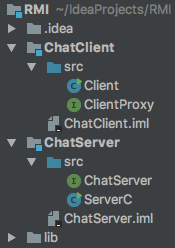
\includegraphics[width=0.2 \linewidth]{images/rmi_ordner}
	\caption{Ordnerstruktur} \label{ordner}
\end{figure} 

Wir implementieren die vorgegebenen Interfaces, also \textbf{ClientProxy} und \textbf{ChatServer}.
\begin{lstlisting}
public interface ClientProxy extends Remote {
    public void receiveMessage (String username, String message) throws RemoteException;
}
\end{lstlisting}
Dieses Interface wird vom Client implementiert und ermöglicht es dem Server die Nachrichten an jeden Client zu verteilen.
\begin{lstlisting}
public interface ChatServer extends Remote {
    public boolean subscribeUser (ClientProxy handle) throws RemoteException;
    public boolean unsubscribeUser (ClientProxy handle) throws RemoteException;
    public void send(String username, String message) throws RemoteException;
}
\end{lstlisting}
ChatServer wird vom Server implementiert und ermöglicht es dem Client sich am Server anzumelden, abzumelden und eine Nachricht zu schicken.

\subsubsection{Server}
Nun implementieren wir als erstes den Server, diese implementiert natürlich das vorher erstellte Interface.
\begin{lstlisting}
public class Server extends UnicastRemoteObject implements ChatServer 
\end{lstlisting}
Als nächstes benötigen wir eine Möglichkeit alle Client zu speichern die sich am Server anmelden, dazu verwenden wir in unserer Abgabe eine \textit{ArrayList}, die nur Objekt vom Typ \textit{ClientProxy} aufnimmt.
\begin{lstlisting}
private ArrayList<ClientProxy> users;
\end{lstlisting}
Jetzt müssen wir diese ArrayList noch instanziieren, dass tun wir im Konstruktor des Servers.
\begin{lstlisting}
public Server() throws RemoteException {
	this.users = new ArrayList<>();
}
\end{lstlisting}

\subsubsubsection{subscribeUser(ClientProxy handle)}

Jetzt müssen wir, da wir das Interface implementieren, die Methoden vom Interface implementieren. Hier beginnen wir mit der Methode \textit{subscribeUser(ClientProxy handle)}. 
\begin{lstlisting}
@Override
public boolean subscribeUser(ClientProxy handle) throws RemoteException {
	System.out.println("Ein User hat sich angemeldet");
	if(users.add(handle))
		return true;
	return false;
}
\end{lstlisting}
Diese Methode bekommt einen Client übergeben, um uns diesen Client zu merken. Wir geben am Server aus das sich ein User anmeldet um alles zu protokollieren. Wir fügen diesen User einfach in die \textit{ArrayList} ein, wenn das funktioniert geben wir ein \textit{true} zurück, andernfalls geben wir ein \textit{false} zurück.

\subsubsubsection{unsubscribeUser(ClientProxy handle)}

Als nächstes implementieren wir die Methode \textit{unsubscribeUser(ClientProxy handle)}.
\begin{lstlisting}
@Override
public boolean unsubscribeUser(ClientProxy handle) throws RemoteException {
	System.out.println("Ein User hat sich abgemeldet");
	if(users.remove(handle))
		return true;
	return false;
}
\end{lstlisting}
Auch hier übergeben wir den Client, der sich abmelden möchte. Wir protokollieren auch hier am Server, dass sich ein User abmeldet. Wir entfernen hier einfach den Client aus der \textit{ArrayList}, welcher sich abmelden möchte, wenn das funktioniert geben wir ein \textit{true} zurück und wenn nicht geben wir ein \textit{false} zurück.

\subsubsubsection{send(String username, String message)}

Jetzt müssen wir noch die letzte Methode implementieren, diese stammt nicht aus den Vorgaben, aber sie ermöglicht es jeden Client, dass dieser eine Nachricht schicken kann. Diese Methode heißt \textit{send(String username, String message)}.
\begin{lstlisting}
@Override
public void send(String username, String message) {
	System.out.println(username + ": " + message);
	
	for(int i = 0; i < users.size(); i++) {
		try {
			users.get(i).receiveMessage(username, message);
		} catch (RemoteException e) {
			e.printStackTrace();		
		}
	}
}
\end{lstlisting}
Diese Methode ruft der Client über RMI auf, diese Methode erwartet den Username des Client und die Nachricht die er senden möchte. Hier protokollieren wir wieder für den Server welcher Client welche Nachricht sendet. Als nächstes gehen wir die komplette \textit{ArrayList} durch und rufen bei jedem Client die Methode \textit{receiveMessage (String username, String message)} auf, dort übergeben wir einfach den Namen vom Client und die Nachricht, der die Nachricht verschickt. Diese Methode hat keine Rückgabe.

\subsubsubsection{main(String[] args)}

Nun benötigen wir nur noch eine \textit{main} Methode um den Server zu starten.
\begin{lstlisting}
public static void main(String[] args) {
	try {
		LocateRegistry.createRegistry(Registry.REGISTRY_PORT);
		ChatServer server = new Server();
		Naming.rebind("ChatServer", server);
		System.out.println("Server wurde gestartet.");
	} catch (Exception e) {
		System.out.println("Server konnte nicht gestartet werden: " + e);
	}
}
\end{lstlisting}
Hier schreiben wir unseren Server in Registry, damit die Client auch auf ihn zugreifen können. Jetzt erstellen wir ein Objekt vom Typen Server und instanziieren ihn auch direkt. Jetzt geben wir jetzt noch unseren Server einen Namen, damit die Clients auch wissen wie sie ihn erreichen können. Als guter Letzt geben wir noch aus das dieser Server gestartet wurde.

\subsubsection{Client}
Auch hier müssen wir das bereits erstellte und vergebene Interface implementieren.
\begin{lstlisting}
public class Client extends UnicastRemoteObject implements ClientProxy
\end{lstlisting}
Nun müssen wir auch hier vorher ein paar Variablen deklarieren.
\begin{lstlisting}
private ChatServer server;

private JTextArea content;
private JTextField message, username;
private JButton connect;
private JFrame frame;
\end{lstlisting}
Die Variable \textit{server} vom Typen \textit{ChatServer} wird benötigt damit wir in den Methoden des Client die Methoden des ChatServer verwenden können. \textit{content} ist eine \textit{JTextArea} und dort wird später unser Chat stattfinden und alle Nachrichten ausgegeben. \textit{message} und \textit{username} sind beide vom Typ \textit{JTextField}. Bei \textit{username} kann der User später seinen Namen angeben damit der Server weiß wie der User heißt und \textit{message} ist dazu da damit der User seine Nachricht schreiben kann. \textit{connect} ist ein \textit{JButton} mit dem kann der User sich mit dem Server verbinden und auch wieder trennen. \textit{frame} ist unser Fenster in dem das komplette GUI dargestellt wird.\\\\Da wir den \textit{server} noch instanziieren müssen benötigen wir einen selbst erstellten Konstruktor.
\begin{lstlisting}
public Client() throws RemoteException {
	this.server = null;
}
\end{lstlisting}

\subsubsubsection{receiveMessage(String username, String message)}

Wir implementiern nun als erstes die Methode vom Interface \textit{ClientProxy}. 
\begin{lstlisting}
@Override
public void receiveMessage(String username, String message) throws RemoteException {
	content.append(username + ": " + message + "\n");
}
\end{lstlisting}
Diese Methode wird vom Server aufgerufen, diese erwartet einen Username und eine Nachricht, sie ist dafür da damit der Server die Nachrichten verteilen kann an die Clients. In dieser Methode hängen wir \textit{content} eine neue Nachricht an, mit dem dazu gehörigen Username der die Nachricht verschickt hat. 

\subsubsubsection{connect()}

Nun kommen noch ein paar interne Methoden, diese haben eine Sichtbarkeit von \textit{private}. Die Methode \textit{connect()} ist dafür da, das sicher jeder Client mit dem Server verbinden kann. 
\begin{lstlisting}
private void connect() {
	if(username.getText().replaceAll(" ", "").length() > 0) {
		try {
			Registry registry = LocateRegistry.getRegistry();
			server = (ChatServer) registry.lookup("ChatServer");

			if(server.subscribeUser(this)) {
				username.setEditable(false);
				connect.setText("Trennen");
			} else {
				JOptionPane.showMessageDialog(frame, "Konnte keine Verbindung herstellen!");
			}
		} catch (Exception e) {
			e.printStackTrace();
		}
	} else {
		JOptionPane.showMessageDialog(frame, "Der Name darf nicht leer sein!");
	}
}
\end{lstlisting}
Wir überprüfen nun als erstes ob ein Username angeben wurde und diese nicht nur Leerzeichen besteht, damit man sich nicht Server verbinden kann, wenn kein Username angeben wurde oder dieser nur aus Leerzeichen besteht. Nun suchen wir nach der vom Server erstellten Registry und setzen den Wert von der vorher instanziierten Variable \textit{server} mit dem auf der Registry liegenden Objekt. Als nächstes melden wir uns als Client selber am Server an, wenn dieses funktioniert hat setzen wir das \textit{username}-Textfield auf nicht editierbar, damit man den Usernamen nicht mehr ändern kann, und ändern den Text vom \textit{connect} auf \textit{Trennen}, damit der User versteht, das man sich nun mit diesem Button wieder abmelden kann, dazu später mehr.

\subsubsubsection{disconnect()}

Diese Methode hat ebenfalls die Sichtbarkeit \textit{private}, da sie nur vom Client intern verwendet wird. Sie ist dazu da damit sich der Client auch wieder vom Server abmelden kann.
\begin{lstlisting}
private void disconnect() {
	try {
		if(server.unsubscribeUser(this)) {
			username.setEditable(true);
			connect.setText("Verbinden");
			content.setText("");
			server = null;
		} else {
			JOptionPane.showMessageDialog(frame, "Abmeldung fehlgeschlagen!");
		}
	} catch (Exception e) {
		e.printStackTrace();
	}
}
\end{lstlisting}
Wir rufen zum abmelden einfach die Methode vom Server auf um uns vom Server abzumelden, wenn dies funktioniert machen wir das \textit{username}-TextField wieder editierbar, setzen den Text vom \textit{connect}-Button wieder auf \textit{Verbinden} damit der User sich wieder neu anmelden kann. Die \textit{content}-TextArea wird zurückgesetzt und setzen den \textit{server} auf \textit{null}, damit wir alles zurückgesetzt haben.

\subsubsubsection{send()}

Wir implementieren nun die letzte interne Methode mit der Sichtbarkeit \textit{private}, diese ist zum senden, der eigentlichen Nachricht an den Server, da.
\begin{lstlisting}
private void send() {
	if (message.getText().replaceAll(" ", "").length() > 0) {
		try {
			server.send(username.getText(), message.getText());
		} catch (RemoteException e) {
			e.printStackTrace();
		}
		message.setText("");
	} else {
		JOptionPane.showMessageDialog(frame, "Nachricht darf nicht leer sein!");
	}
}
\end{lstlisting}
Diese Methode überprüft ob die eingegebene Nachricht nicht leer ist oder nicht nur aus Leerzeichen besteht, wenn das zutrifft sendet der Client die Nachricht mit dem dazugehörigen Username an den Server und dieser verteilt diese dann an alle Clients. Wir setzen das \textit{message}-TextField zurück, damit der User seine Nachricht nicht direkt öfter hintereinander schicken kann.

\subsubsubsection{initUI()}

Diese Methode erstellt das User-Interface für den Client. Diese Funktion ruft alle internen Funktionen auf, deswegen muss sie zwingend aufgerufen werden. Als erstes erstellen wir diese Methode.
\begin{lstlisting}
public void initUI(){
	...
}
\end{lstlisting}
Jetzt müssen wir die ganzen Komponenten die wir verwenden wollen instanziieren.
\begin{lstlisting}
frame=new JFrame("Client");
JPanel main =new JPanel();
JPanel top =new JPanel();
JPanel cn =new JPanel();
JPanel bottom =new JPanel();
message =new JTextField();
username =new JTextField();
content =new JTextArea();
connect=new JButton("Verbinden");
JButton send=new JButton("Senden");
\end{lstlisting}
\textit{frame} ist wie bereit oben erwähnt unseres Hauptfenster. \textit{main} ist unsere Hauptpanel, dort fügen wir alle anderen Panel ein. \textit{top} ist das Panel für das \textit{username}-TextField und \textit{connect}-Button. \textit{cn} ist das Panel wo die \textit{content}-TextArea und eine ScrollBar eingebunden werden soll.Das\textit{bottom} Panel ist für das \textit{message}-TextField und den \textit{send}-Button.\\\\Die Anordnung der ganzen kann wie gewünscht gemacht werden und wird hier nicht weiter drauf eingegangen.\\\\Nun müssen wir noch \textit{ActionListener} hinzufügen damit wir auf die Buttons und TextFields reagieren können. Wir fangen mit den \textit{ActionListener} für den \textit{connect}-Button an.
\begin{lstlisting}
connect.addActionListener(e -> {
	if(connect.getText().equalsIgnoreCase("verbinden")) {
		connect();
	} else {
		disconnect();
	}
});
\end{lstlisting}
Wir überprüfen nun als erstes den Text vom \textit{connect}-Button und wenn diese gleich \textit{Verbinden} ist, rufen wir die private Methode \textit{connect()} auf, wenn nicht dann rufen wir \textit{disconnect()}. Das selbe tun wir für den \textit{ActionListener} von \textit{username}-Textfield.
\begin{lstlisting}
username.addActionListener(e -> {
	if(connect.getText().equalsIgnoreCase("verbinden")) {
		connect();
	} else {
		disconnect();
	}
});
\end{lstlisting}
Nun müssen wir das selbe für den \textit{send}-Button und das \textit{message}-TextField tun.
\begin{lstlisting}
message.addActionListener(e -> {
	send();
});

send.addActionListener(e -> {
	send();
});
\end{lstlisting}
Wenn wir das nun ausführen würden, würde sich ein GUI öffnen, siehe \autoref{gui}
\begin{figure}[H]
	\centering
	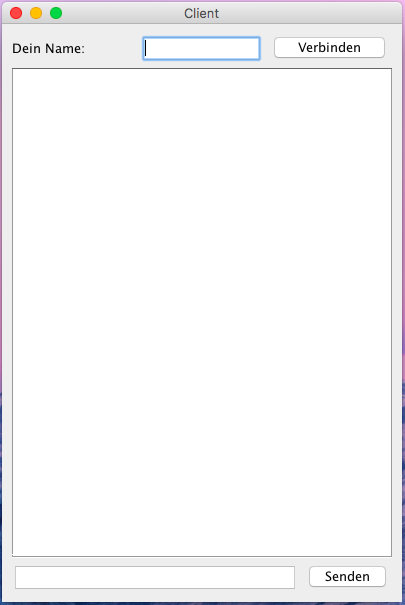
\includegraphics[width=0.2 \linewidth]{images/rmi_gui}
	\caption{Chat GUI} \label{gui}
\end{figure} 

\subsubsubsection{main(String[] args)}
Nun müssen wir den Client noch ausführbar machen, deswegen machen wir noch eine \textit{main}-Methode.
\begin{lstlisting}
public static void main(String[] args) {
	Client c = null;
	try {
		c = new Client();
	} catch (RemoteException e) {
		e.printStackTrace();
	}
	c.initUI();
}
\end{lstlisting}
Als erstes deklarieren wir einen Client, diesen instanziieren wir als nächstes in einem \textit{try}. Jetzt rufen wir mit dem Client nur noch das GUI auf. 

\subsection{Fazit}
Diese Aufgabe war ziemlich umfangreich, aber relativ einfach umzusetzen mit der dazugehörigen Vorlesung. Anfangs gab es Verständnisprobleme mit RMI, diese wurden aber mit der Grafik auf dem Aufgabenblatt weggeräumt.




